\section{AMCL中odom的数据处理}



\begin{frame}{参数配置}
  AMCL关于odom的参数配置列表(以差速模型为例):

  % \frametitle{表格}
  \begin{table}[htbp!]
    \centering
    % \caption{}
    \begin{tabular}{c|c|c}
      \toprule[1pt]
      参数	& 默认值 & 描述  \\
      \toprule[1pt]
      odom\_model\_type	& diff & 里程计运动模型,种类有diff、ommi等 \\
 	    \hline
      odom\_alpha1	&  0.2 & 机器人旋转分量中的旋转噪声 \\
      \hline
      odom\_alpha2	&  0.2 & 机器人平移分量中的旋转噪声 \\
      \hline
      odom\_alpha3	&  0.2 & 机器人平移分量中的平移噪声 \\
      \hline
      odom\_alpha4	&  0.2 & 机器人旋转分量中的平移噪声 \\
 	    \bottomrule[1pt]
    \end{tabular}
  \end{table}
\end{frame}

\begin{frame}
  \frametitle{里程计运动模型(一)}
  \begin{itemize}
    \item 在计算时间$\Delta t$内,控制$u_t = (\nu, \omega)$ 作用下将机器人位姿从$x_{t-1} = (x, y, z)^T$ 
          变成位姿$x_t = (x^\prime, y^\prime, \theta^\prime)^T$ 的概率$p(x_t | u_t, x_{t-1})$ 。
    \item 为了保持状态空间比较小,通常把里程计数据认为是控制信号。
    \item 总之,用距离测量代替控制, 距离是通过里程计编码信息得到的。
  \end{itemize}

\end{frame}



% \begin{frame}
%   % 里程计差分模型:两平行轮作驱动,另外附加一个万向轮作支撑。
% % 的
%   % 在AMCL算法中将机器人的每一步的广义运动进行了拆解,拆解成包含三个动作的序列:
%   \begin{figure}[!h]
%     \centering
%     % Requires \usepackage{graphicx}
%     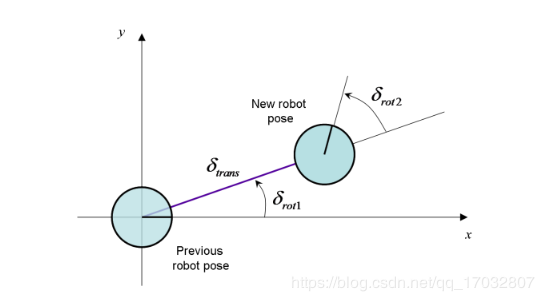
\includegraphics[width=2cm]{amcl/odom_model}\\
%     \caption{logo图片样例}\label{pic6}
%   \end{figure}
% \end(frame)

% \begin{frame}{参数配置}
%   里程计差分模型:两平行轮作驱动,另外附加一个万向轮作支撑。

%   在AMCL算法中将机器人的每一步的广义运动进行了拆解,拆解成包含三个动作的序列:

%   \begin{itemize}
% 		\item 在起始点旋转,转向终止点的方向
% 	 	\item 着该方向做直线运动到终止点
% 	 	\item 在终止点进行旋转,转到目标方向
% 	 \end{itemize}
%   \begin{figure}[!h]
%     \centering
%     % Requires \usepackage{graphicx}
%     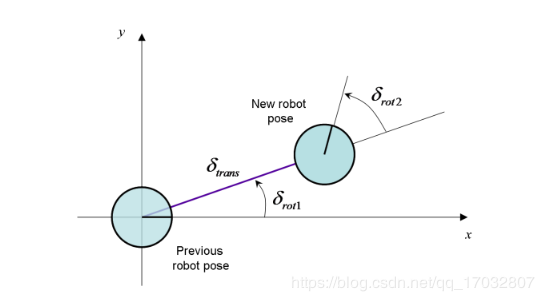
\includegraphics[width=4cm]{amcl/odom_model.png}\\
%     \caption{logo图片样例}\label{pic6}
%   \end{figure}
%   \end{frame}

  \begin{frame}{里程计运动模型(二)}
    
    \begin{columns}%0.6 0.4表示相对比例
    \column{0.5\textwidth}%<1->
    % \frametitle{条目}
    \begin{itemize}
    \item 里程计差分模型:两平行轮作驱动,另外附加一个万向轮作支撑。
    \item 在AMCL算法中将机器人的每一步的广义运动进行了拆解,拆解成包含三个动作的序列:
      \begin{itemize}
        \item 在起始点旋转,转向终止点的方向
         \item 朝着该方向做直线运动到终止点
         \item 在终止点进行旋转,转到目标方向
      \end{itemize}

    \end{itemize}

    \column{0.5\textwidth}%<1->
    % 分栏的右侧插入了图片。
     \begin{figure}[!h]
      \centering
      % Requires \usepackage{graphicx}
      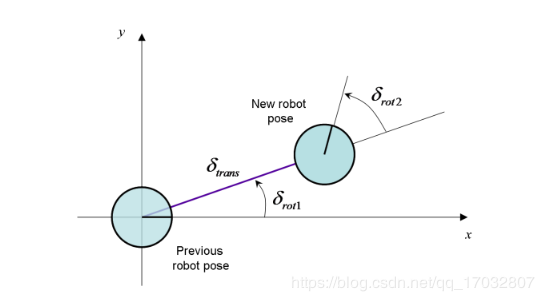
\includegraphics[width=5cm,trim=50 25 50 50,clip]{amcl/odom_model}\\
      % \caption{logo图片样例}\label{pic6}
    \end{figure}
    \begin{itemize}
      \item $\delta_{rot1}$代表在起始点的旋转
      \item $\delta_{trans}$代表着第二段平移过程
      \item $\delta_{rot2}$代表着在终止点的旋转
    \end{itemize}
    \end{columns}
    % 分栏后面的一些内容!!
    \end{frame}

\begin{frame}{里程计的噪声}
  % \begin{itemize}
	% 	\item 在起始点旋转,转向终止点的方向
	%  	\item 着该方向做直线运动到终止点
	%  	\item 在终止点进行旋转,转到目标方向
  %  \end{itemize}
  \begin{itemize}
  \item 里程计无噪声情况 --- 里程计读轮子的转圈和机器人的位移是精确对应的。
  \item   理论和仿真可以做到,假设:
    \begin{itemize}
      \item 轮子与地面不打滑
      \item 地面绝对平整
      \item 轮子不变形
      \item 里程计和机器人轮轴之间没有迟滞可以做到完全时间同步,等等
    \end{itemize}
  \item 在AMCL中,里程计是作为状态预测器存在的,根据控制信息和上一时刻机器人的状态,同时考虑里程计噪声信息,对当前时刻状态进行预测。
  \end{itemize}
\end{frame}  


\begin{frame}[fragile]
  \frametitle{采样算法}

  % \begin{algorithm}[htb]  
    % \caption{Title}  
    % \label{alg:Framwork}  
    % \begin{algorithmic}  
    %   \Require  
    %   xxxxxxxx 
    %   \Ensure  
    %  xxxxxxxxx
    %     \For{xyz}
    %     \If {yyyyyyy}  
    %     \State asdfghjkl;
    %     \Else
    %     \State qwertyuiop;
    %      \If{zzzzzzz}
    %            \State zxcvbnm;
    %      \EndIf
    %     \EndIf
    %  \EndFor  
    %   \For {abc }  
    %     \State qazwsxedc; 
    %   \EndFor
    % \end{algorithmic}  
  % \end{algorithm}

  % \begin{algorithm} 
    % \caption{UKF\_MCL算法}
    \begin{algorithmic}[frame = shadowbox]
        \State Algorithm sample\_motion\_model\_odometry$(u_t, x_{t-1})$ :
        \State $\delta_{rot1} = atan2(\delta_x, \delta_y) - \theta_{old}$
        \State $\delta_{trans} = \sqrt{\delta_x^2 + \delta_y^2}$
        \State $\delta_{rot2} = \delta_\theta - \delta_{rot1}^2$

        \State $\hat{\delta}_{rot1} = \delta_{rot1} - smaple(\alpha_1 \delta_{rot1}^2 + \alpha_2 \delta_{trans}^2)$
        \State $\hat{\delta}_{trans} = \delta_{trans} - smaple(\alpha_3 \delta_{trans}^2 + \alpha_4 \delta_{rot1}^2 + \alpha_4 \delta_{rot2}^2)$
        \State $\hat{\delta}_{rot2} = \delta_{rot2} - smaple(\alpha_1 \delta_{rot2}^2 + \alpha_2 \delta_{trans}^2)$

        \State $x^\prime = x + \hat{\delta}_{trans} \cos(\theta + \hat{\delta}_{rot1})$
        \State $y^\prime = y + \hat{\delta}_{trans} \sin(\theta + \hat{\delta}_{rot1})$
        \State $\theta^\prime = \theta + \hat{\delta}_{rot1}  + \hat{\delta}_{rot2}$

        \State return $x_t = (x^\prime, y^\prime, \theta^\prime)^T$

    \end{algorithmic}
  % \end{algorithm}

\end{frame}


\begin{frame}
  \frametitle{Box-Muller变换}

  Box-Muller变换是通过服从均匀分布的随机变量,来构建服从高斯分布的随机变量的一种方法。
  具体的描述为:选取两个服从[0,1]上均匀分布的随机变$x_1$, $x_2$, $y_1$, $y_2$满足

  % \begin{equation}
  %   \begin{cases}
  %     y_1 = \cos(2 \pi x_2) \sqrt{-2 \ln{x_1}} \\
  %     y_2 = \sin(2 \pi x_2) \sqrt{-2 \ln{x_1}}
  %   \end{cases}
  % \end{equation}

  \begin{equation}
    \begin{cases}
      y_1 = \frac{x_1}{\sqrt{w}} \sqrt{-2 \ln{w}} \\
      y_2 = \frac{x_2}{\sqrt{w}} \sqrt{-2 \ln{w}}
    \end{cases}
  \end{equation}

  其中,$w = x_1^2 + x_2^2$,$y_1$和$y_2$是服从$N(0,1)$分布的随机数;

  代码实现里面取的是$y_2$,并且在$y_2$前面乘以sigma,获得N(0, sigma)分布的随机数。

\end{frame}

\begin{frame}[fragile]
  \frametitle{Odom代码分析(一)}
  \begin{lstlisting}[frame=shadowbox]  
    double pf_ran_gaussian(double sigma)
    {
      double x1, x2, w, r;
      do
      {
        do { r = drand48(); } while (r==0.0);
        x1 = 2.0 * r - 1.0;
        do { r = drand48(); } while (r==0.0);
        x2 = 2.0 * r - 1.0;
        w = x1*x1 + x2*x2;
      } while(w > 1.0 || w==0.0);

      return(sigma * x2 * sqrt(-2.0*log(w)/w));

  \end{lstlisting}
\end{frame}


\begin{frame}[fragile]
  \frametitle{Odom代码分析(二)}

  入口函数:

  \begin{lstlisting}[frame=shadowbox]
    bool AMCLOdom::UpdateAction(pf_t *pf, AMCLSensroData *data);
  \end{lstlisting}

  计算 $\delta_{rot1}$、$\delta _{rot2}$和$\delta _{trans}$:
  \begin{lstlisting}[frame=shadowbox]
    ndata = (AMCLOdomData*) data;

    if (sqrt(ndata->delta.v[0]*ndata->delta.v[0] + ndata->delta.v[1]*ndata->delta.v[1]) < 0.01) 
      delta_rot1 = 0.0;
    else
      delta_rot1 = angle_diff(atan2(ndata->delta.v[1], ndata->delta.v[0]), old_pose.v[2]);
      
    delta_trans = sqrt(ndata->delta.v[0]*ndata->delta.v[0] + ndata->delta.v[1]*ndata->delta.v[1]);
    delta_rot2 = angle_diff(ndata->delta.v[2], delta_rot1);
  \end{lstlisting}


\end{frame}


\begin{frame}[fragile]
  \frametitle{代码分析(三)}
  \begin{lstlisting}[frame=shadowbox]
    delta_rot1_noise = std::min(fabs(angle_diff(delta_rot1, 0.0)), fabs(angle_diff(delta_rot1, M_PI)));
    delta_rot2_noise = std::min(fabs(angle_diff(delta_rot2, 0.0)), fabs(angle_diff(delta_rot2, M_PI)));

    for(int i=0; i<set->sample_count; i++)
    {
      pf_sample_t* sample = set->samples + i;
      delta_rot1_hat = angle_diff(delta_rot1, pf_ran_gaussian(alpha1_*delta_rot1_noise*delta_rot1_noise + alpha2_*delta_trans*delta_trans));
      delta_rot2_hat = angle_diff(delta_rot2, pf_ran_gaussian(alpha1_*delta_rot2_noise*delta_rot2_noise + alpha2_*delta_trans*delta_trans));
      delta_trans_hat = delta_trans - pf_ran_gaussian(alpha3_*delta_trans*delta_trans + alpha4_*delta_rot1_noise*delta_rot1_noise + alpha5_*delta_rot2_noise*delta_rot2_noise);
  \end{lstlisting}
\end{frame}

\begin{frame}[fragile]
  \frametitle{代码分析(四)}
  \begin{lstlisting}[frame=shadowbox]
      sample->pose.v[0] += delta_trans_hat * cos(sample->pose.v[2] + delta_rot1_hat);  
      sample->pose.v[1] += delta_trans_hat * sin(sample->pose.v[2] + delta_rot1_hat);  
      sample->pose.v[2] += delta_rot1_hat + delta_rot2_hat;
    }
  \end{lstlisting}
\end{frame}